%!TEX TS-program = pdflatex
%!TEX root = tesi.tex
%!TEX encoding = UTF-8 Unicode


     %%%%%%%%%%%%%%%%%%%%
     %                  %
     %  capitolo1.tex   %
     %                  %
     %%%%%%%%%%%%%%%%%%%%

\chapter{Introduction to Time Series Data}

\section{What is time series data?}
Time series data can be thought of as a series of data points, measuring a certain variable
over time, stored in time order. Time series datasets most commonly share three
characteristics \cite{AjayKulkarni2018What} :
\begin{itemize}
	\item Data points are almost always stored as a new record
	\item Data typically arrive in time order
	\item Time is the most important feature of time series data and is a key attribute that distinguishes it from other data
\end{itemize}

For example, let us consider the S\&P 500, a stock market index based on the market
capitalization of the largest 500 companies in the USA. We are interested in collecting the high, low and
closing price on a daily basis. The resulting data set is illustrated in Figure~\ref{sp500}.

\begin{figure}
\begin{center}
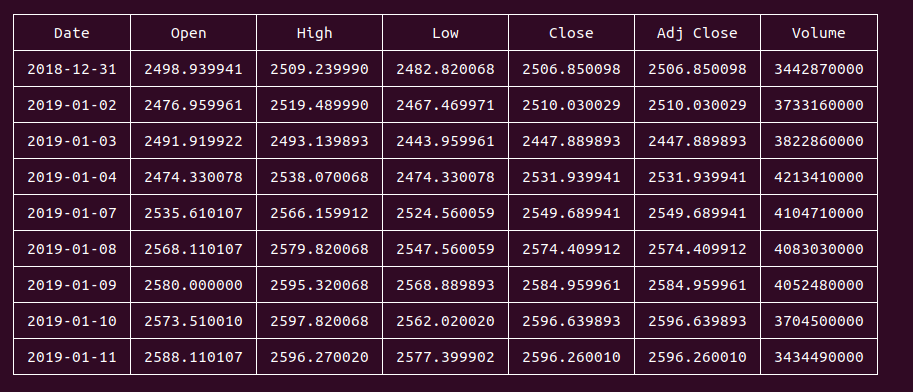
\includegraphics[width=400pt]{sp500}
\caption[sp500]{Time series values for the S\&P 500 aggregated on a daily basis}
\label{sp500}
\end{center}
\end{figure}

The date column is the time index, while the other columns represent measurements of some
specific metrics. This is a typical example of time series data, although not every dataset
containing date/time information is necessarily a time series data set.

The rule of thumb is that with time series data sets changes over time are tracked by creating
new records, rather than updating existing ones. If you have a record with a timestamp, and
whenever something changes in the measurement you create a new record instead of updating the
previous one, then you have a time series dataset.


\section{What is the importance of time series data?}
Time series data is becoming increasingly important in our world, as one can infer from the
growing popularity of time series databases in the period 2017-2019 (Figure~\ref{tspopularity}).

\begin{figure}
\begin{center}
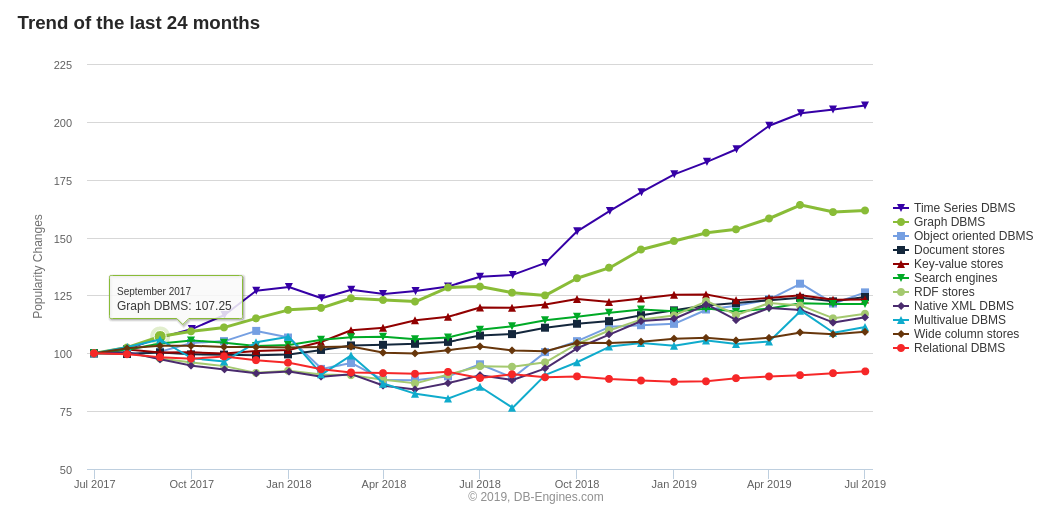
\includegraphics[width=400pt]{tspopularity}
\caption[tspopularity]{Database popularity in the period 2017-2019 according to
\url{https://db-engines.com}, July 2019}
\label{tspopularity}
\end{center}
\end{figure}

Many different businesses rely on the collection and the analysis of this type of data.
DevOps monitoring, scientific measurements, financial markets are just a few business sectors
heavily using time series data.  In most of the applications relying on time series data, it
is vital to collect values as often as possible, to create faster and more accurate monitoring
systems, better models and simulations, more accurate forecasting predictions. As an example,
consider a system that monitors the overall CPU usage of a distributed system. Whenever the
CPU usage exceeds a certain threshold, a remediation action is triggered (for example spawning
an additional node to reduce the load on the system). It is apparent that the usefulness of
the system depends on how often the CPU usage values are collected (the more frequently values are collected, the faster the detection of some anomaly and the faster the remediation action can take place).

The need for finer temporal resolutions requires automatically storing larger quantities of
data, up to the point where traditional relational database systems are not able to handle
the scale. This is because relational database systems store data as a collection of
fixed-size pages on disk. Data is usually indexed by data structures that minimize disk
access, most commonly B-trees. When data sets become large to the point it is not possible
to store indexes in memory anymore, inserting or updating a row might require swapping index
pages from memory to disk, which drastically decreases performance
\cite{Freedman2017Timeseries}. For this reason, new databases that specifically target
time series data have been created. These databases have higher ingestion rates, faster
queries at scale and better data compression as compared to traditional RDBMS. In this
dissertation, I will analyze the problem of data compression in time series data.

\section{Why compressing time series?}
Finding a good compression algorithm to store time series can have multiple benefits depending
on the adopted technique and the use case.
Intuitively, reducing the storage needs of an application allows the system to increase the 
temporal resolution at which the data is recorded.
The storage requirements may be reduced up to the point the whole data set can fit in memory,
reducing writing and reading latency by an order of magnitude or more.
If the application is network bound, compressing data means reducing the amount of data to be
transferred from server to client or the other way around.
In some IoT applications, the compression can be done at the device level, so that less data
need to be transferred over the network. This is usually more power efficient, as the energy
required to compress the data is much less compared to the energy required to transmit it.

\section{Four approaches for time series compression}
We can identify four different approaches for compressing time series data.
\begin{enumerate}
	\item \textbf{Storing aggregates}. In most applications, we are mostly interested in
	recent data as compared to older data. Thus, older data can be $``$aged out$"$ , that is,
	stored in aggregates over a longer temporal interval. Consider the previous example of
	the S\&P Index stock price. Stock prices of the current year can be aggregated over a
	one-hour interval, while older data can be aggregated over days, weeks, and even months.
	One problem with this approach is that aggregates remove fluctuations and outliers that
	are sometimes important when analyzing historical data.
	\item \textbf{Lossless compression}.\ Time series data is characterized by some properties
	that can be exploited to obtain good compression ratios.  For example, most of the time
	data comes at regular intervals, so it does not make sense to store the whole timestamp
	value for each record, but rather go with a delta encoding approach, that is storing only
	the difference between sequential timestamps.
	\item \textbf{Lossy compression. }Many applications are concerned with the trends that
	can be extracted from time series data, and do not require a high level of accuracy. For
	this type of applications, lossy compression can be considered, which usually results in
	much better compression rates as compared to lossless compression.
	\item \textbf{General-purpose algorithms}. Some time series databases do not offer
	compression out of the box. In these cases, one can consider running the databases on
	ZFS or other file systems that offer data compression \cite{A2019TimescaleDB}. Other
	benchmarks \cite{Danjou2016Timeseries} have indicated that general-purpose algorithms
	such as LZ4, achieve good compression ratios and may be more desirable to custom solutions
	given their highly efficient implementations.
\end{enumerate}